To evaluate our state estimation, we compare approaches and parameter sensitivities with respect to the accuracy, robustness and flexibility requirements defined in section \ref{sec:design-requirements}. We use real measurement data from previous testing sessions with the \gls{dv} vehicle, recorded directly from the \gls{can} bus, making the evaluation realistic. We embed the state estimation into a simulation environment, which loads the measurement data and feeds them into the state estimation model. It also generates signals for the time since the arrival of the last measurement based on the signal frequency, since these are not included in the measurement data. Additionally, sensor failures can be injected.


\section{Results}
A fundamental problem with evaluation of state estimations is the lack of ground truth data, which only a vehicle simulation could provide. Since we do not have access to one, we resort to a visual inspection based on physical knowledge. For the \gls{ekf}, we additionally analyze the residuals, since non-zero mean residuals indicate a model--reality mismatch~\cite[p.~158]{AlexanderWischnewski.2019}. We will now show simulation results from all three stages of the state estimation.


\subsection{IMU Fusion}
The \gls{imu} fusion is the only part of the preprocessing stage we will evaluate, since everything else is straightforward physical transformations. Figure \ref{fig:imu-fusion} shows the input measurements from two \glspl{imu} mounted about \SI{80}{\centi\meter} in front and behind \gls{cog} (see section \ref{sec:design-sensor-setup}) as well as the result of their mean-based fusion. The maximum-likelihood-based fusion does not work with the above setup since singular matrices occur, but after adjusting the position parameters for the algorithm to have a small non-zero $y$-position, it gives the same results as the mean-based fusion for $a_x$, $a_y$, $\dot{\psi}$ and $\ddot{\psi}$. Notice how the fusion result is effectively the mean of both inputs and still rather noisy, despite being somewhat reduced. The full measurements and fusion results can be found in appendix \ref{sec:appendix-imufusion}.

\begin{figure}[t]
	\centering
	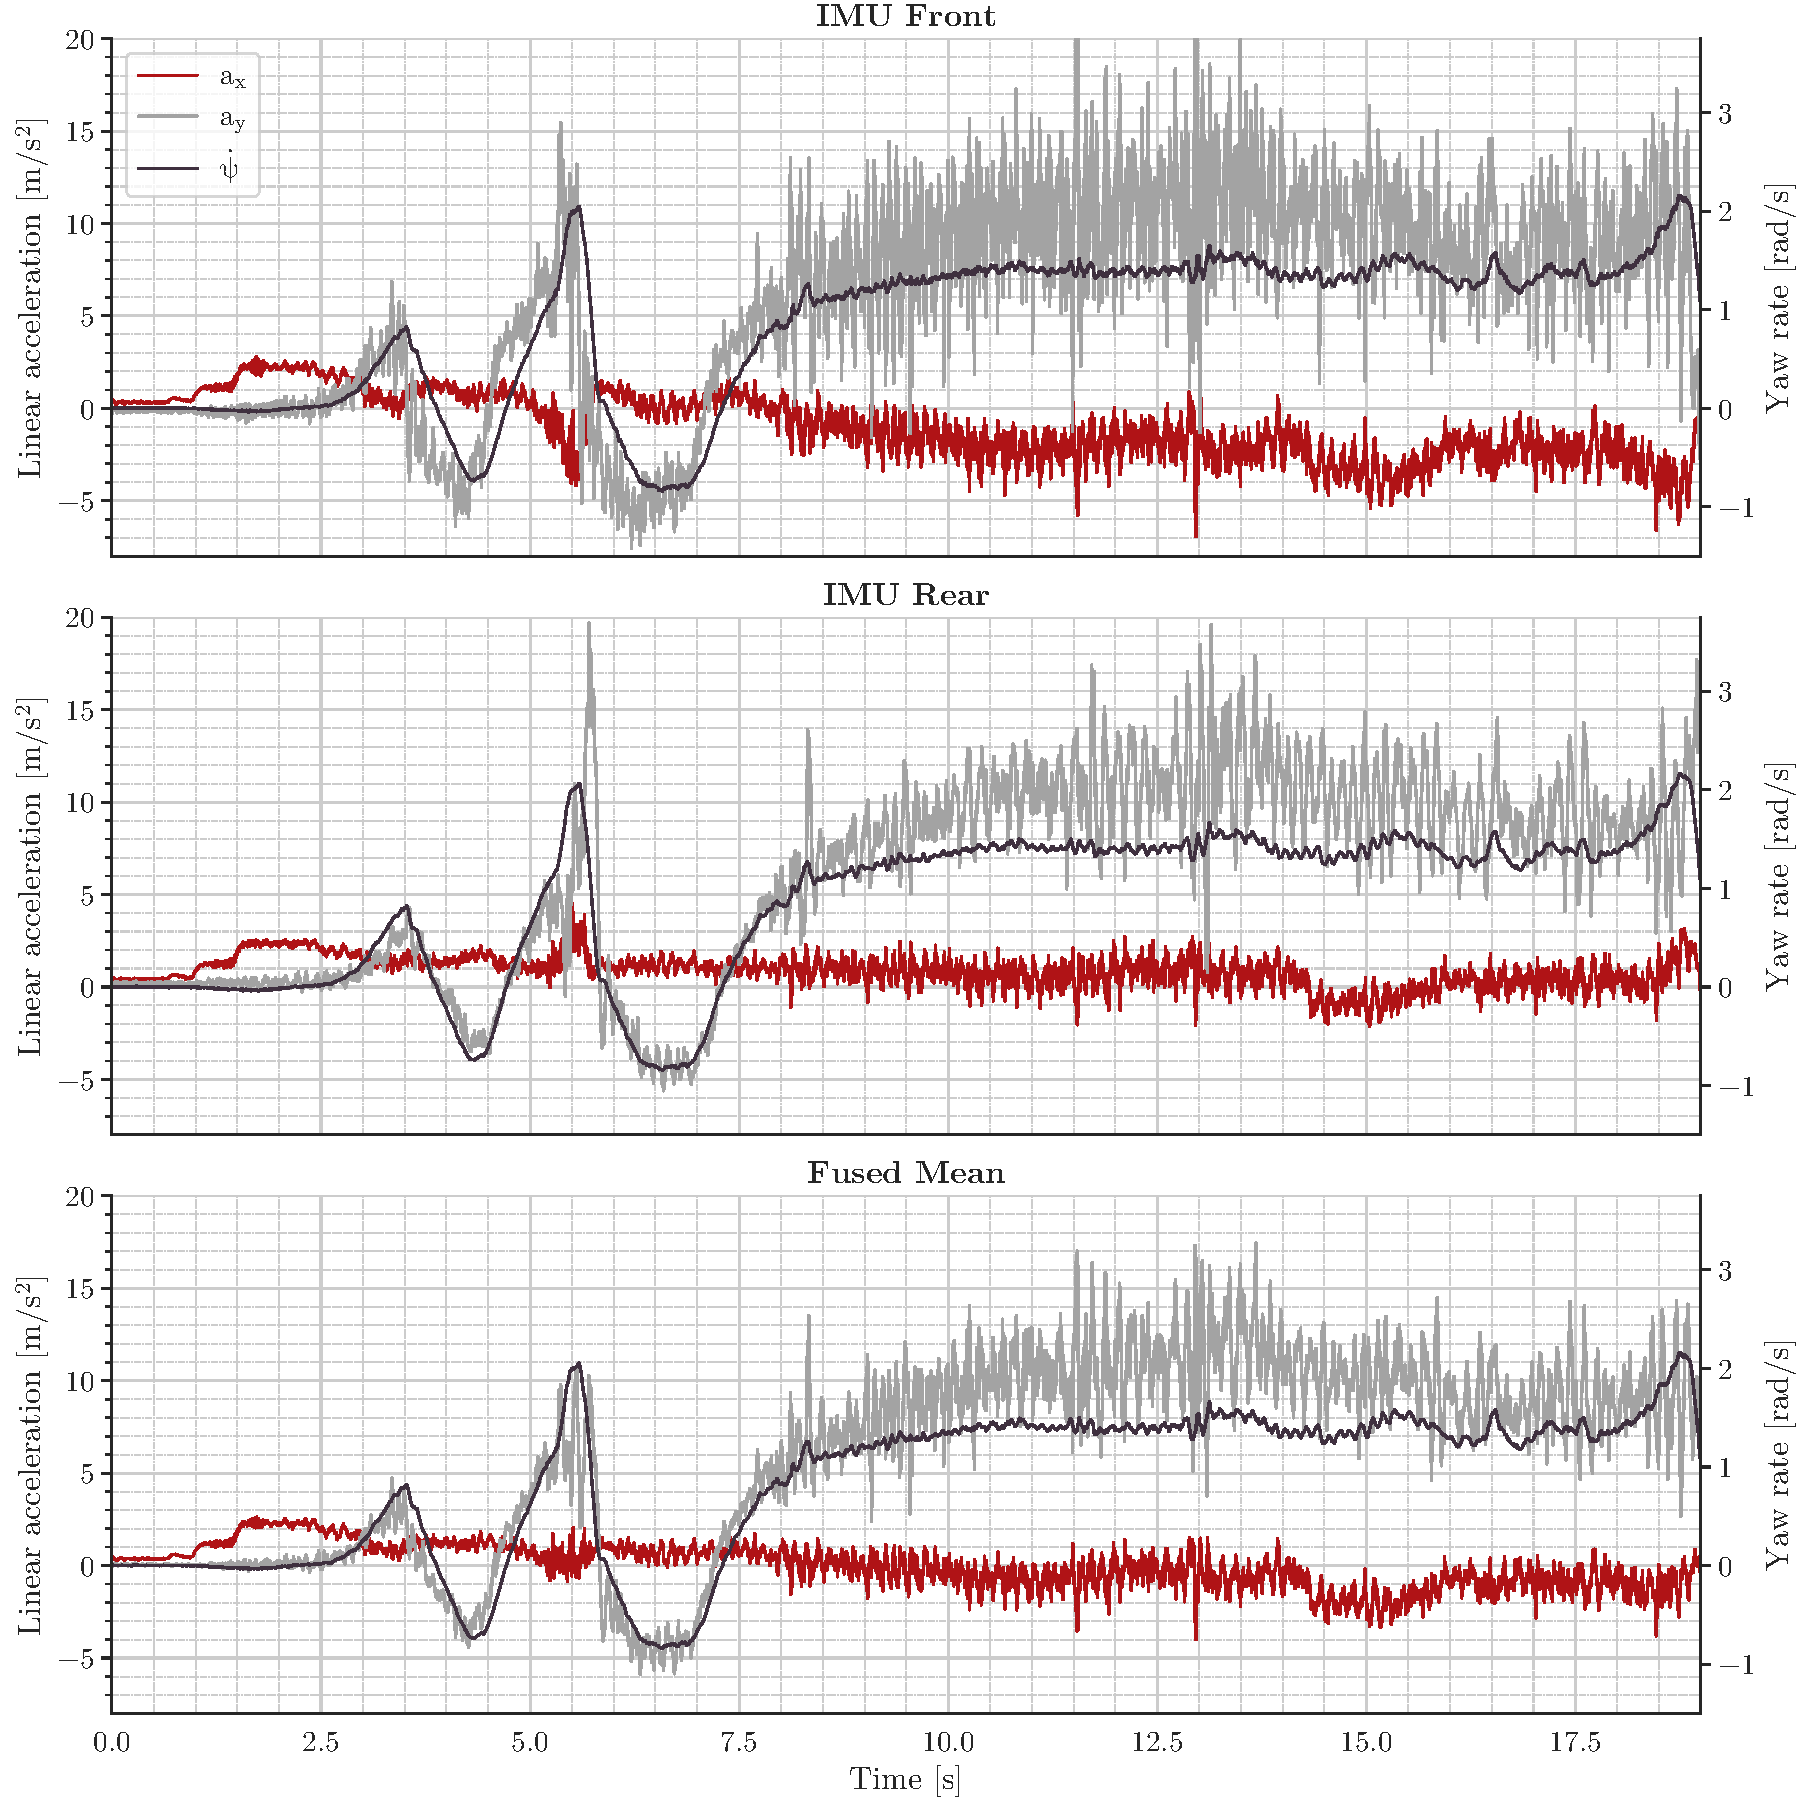
\includegraphics[width=\textwidth]{plot_imu_fusion}%
	\caption{IMU measurements and fusion results}
	\label{fig:imu-fusion}
\end{figure}


\subsection{Failure Detection}
The effect of the failure detection on the state estimate is shown in figure \ref{fig:failure-detection} for the velocity estimate. The measurement of the optical velocity sensor has a null at around \SI{400}{\milli\second} and two less severe outliers before. The sanity check detects transients through the maximum plausible difference of consecutive samples. It reacts quickly but cannot detect persistent outliers such as the null. The \gls{ekf} bank does not detect the two outliers at the beginning, but excels at detecting the persistent null. Notice how the estimate of much more stable and robust to failures with the failure detection, since the faulty measurements are disabled in the \gls{ekf} and other sensors and the model prediction are used. The stability increases when enabling debouncing with a time of \SI{50}{\milli\second}.

\begin{figure}[t]
	\centering
	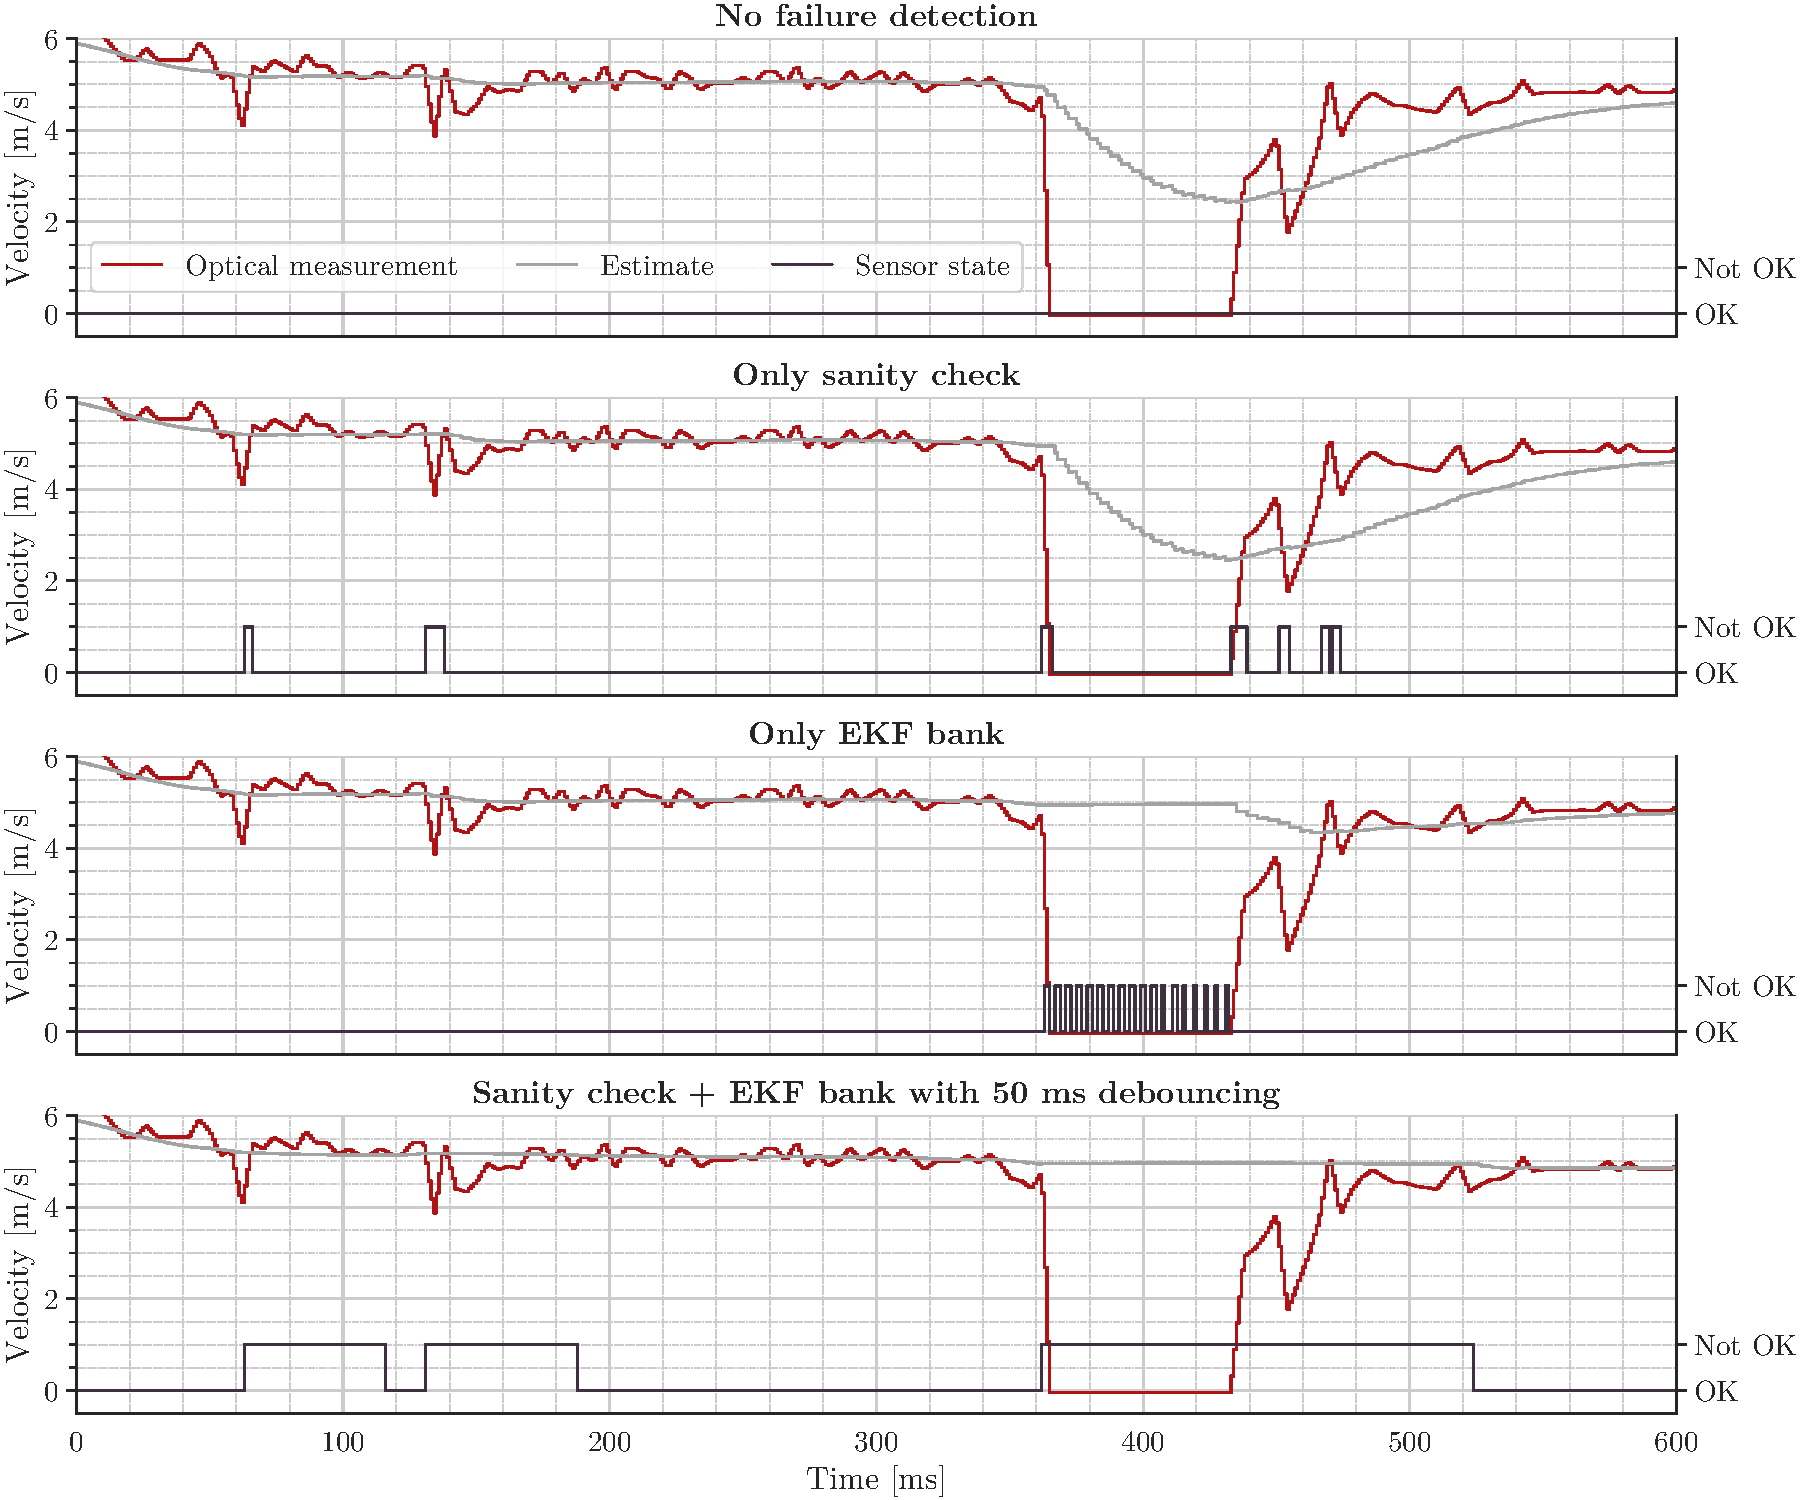
\includegraphics[width=\textwidth]{plot_failure_detection}%
	\caption{Different failure detection modes}
	\label{fig:failure-detection}
\end{figure}

Figure \ref{fig:failure-detection-nssr} shows how large residuals are generated for the \gls{ekf} instances of the bank that do not include the optical sensor. When both \glspl{nssr} cross the threshold, the measurement of the optical sensor is marked as failure. When only one \glspl{nssr} crosses the threshold, an outlier cannot be confidently detected. The measurements and \glspl{nssr} of all three velocity sensors for this example can be found in appendix \ref{sec:appendix-failure-detection}. The intermittency of the residuals stems is a result of the difference of \gls{vdc} execution rate and measurement rates.

\begin{figure}[t]
	\centering
	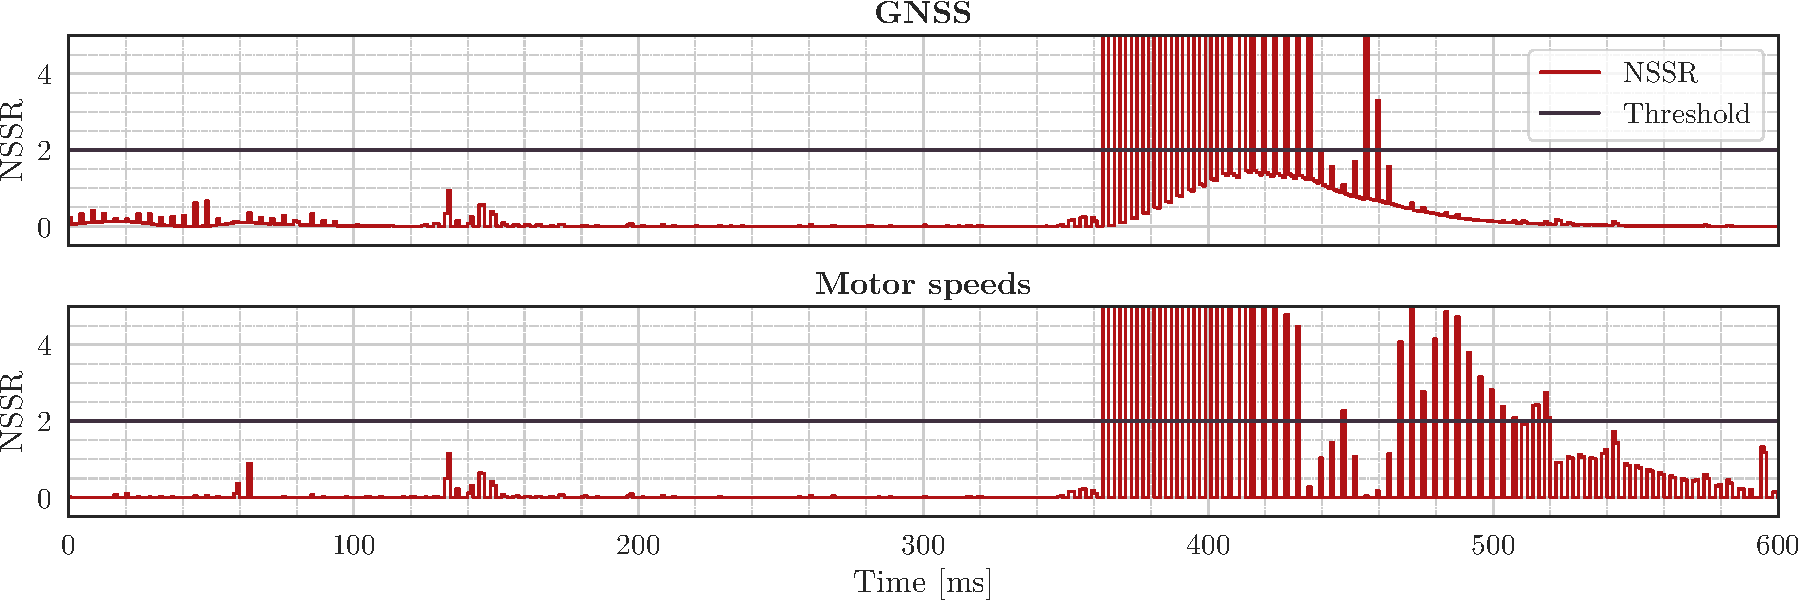
\includegraphics[width=\textwidth]{plot_failure_detection_nssr}%
	\caption{Normalized sums of squared residuals of EKF bank}
	\label{fig:failure-detection-nssr}
\end{figure}

The configuration of thresholds and debouncing time has a large impact on failure detection performance. The choice of parameters is always a tradeoff between false positives and false negatives. For example, the \gls{ekf} bank would have recognized the two outliers with a lower threshold, but would be much more prone to noise. Furthermore, a long debouncing time means that a sensor has more time to recover, but that the \gls{ekf} relies only on the model during that time.


\subsection{EKF}
The estimated longitudinal and lateral velocities from the \gls{ekf} with failure detection are shown in figure \ref{fig:ekf-velocities}. They have much less noise than the sensor measurements and are generally not affected by failures such as spikes in the motor speeds at \SI{5.5}{\second} or the outliers of the optical sensor at \SI{16}{\second}. The residuals for the longitudinal velocity have a mean of zero, which means that predictions match the measurements well, and are low even then the optical sensor is disabled. However, the estimated lateral velocity generally has a lower absolute value than the measurement, which could indicate an inaccurate model. This is especially obvious when disabling the optical sensor, as would be the case in the \gls{dv}. All \gls{ekf} estimates and their residuals can be found in appendix \ref{sec:appendix-ekf}.

\begin{figure}[t]
	\centering
	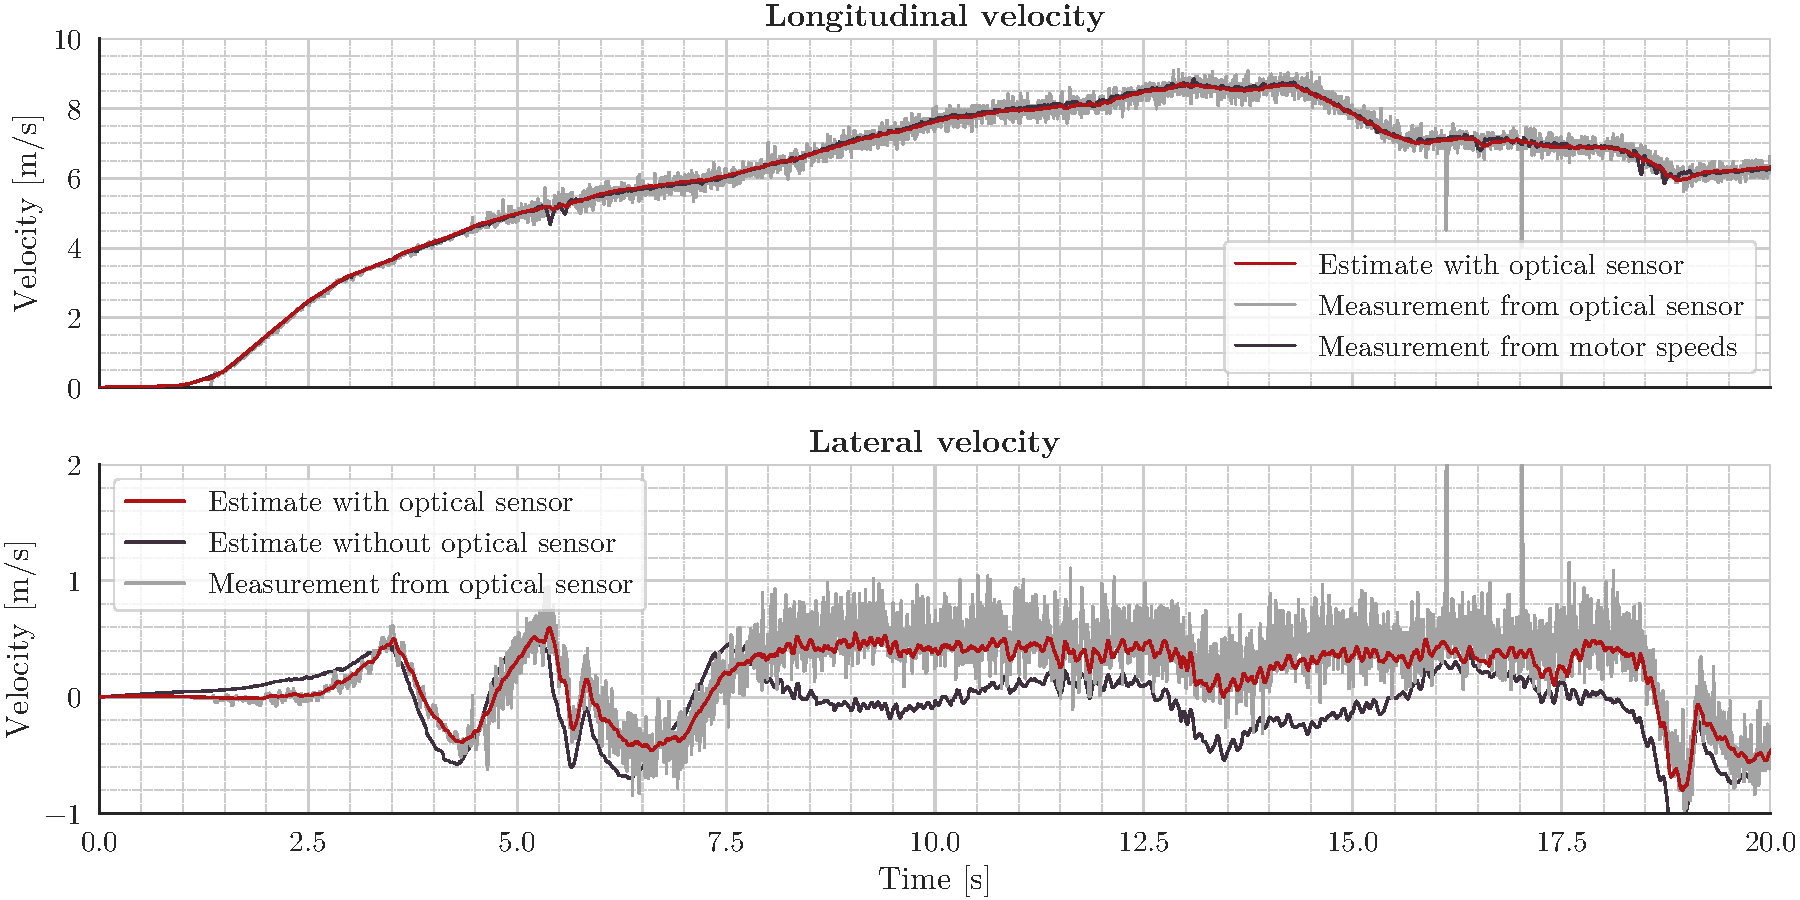
\includegraphics[width=\textwidth]{plot_ekf_velocities}%
	\caption{EKF estimate for velocities}
	\label{fig:ekf-velocities}
\end{figure}

The quality of the position estimate depends strongly on the knowledge of the heading, since it related the velocity to the predicted position. Heading measurements are only available in the \gls{dv}, but were not available for evaluation. Therefore we compare the estimates without an initial heading, i.e. $\psi_0 = 0$, and with an initial heading guessed from the vehicle's movement in figure \ref{fig:ekf-position}. The estimate follows the measurement much more closely in the latter case, with lower residuals than when no initial heading is known (see appendix \ref{sec:appendix-ekf}). The heading itself, normalized to be between $-\pi$ and $\pi$, comes only from the prediction using the yaw rate and is not corrected by measurements. Note that the initial heading is usually not known.

\begin{figure}[t]
	\centering
	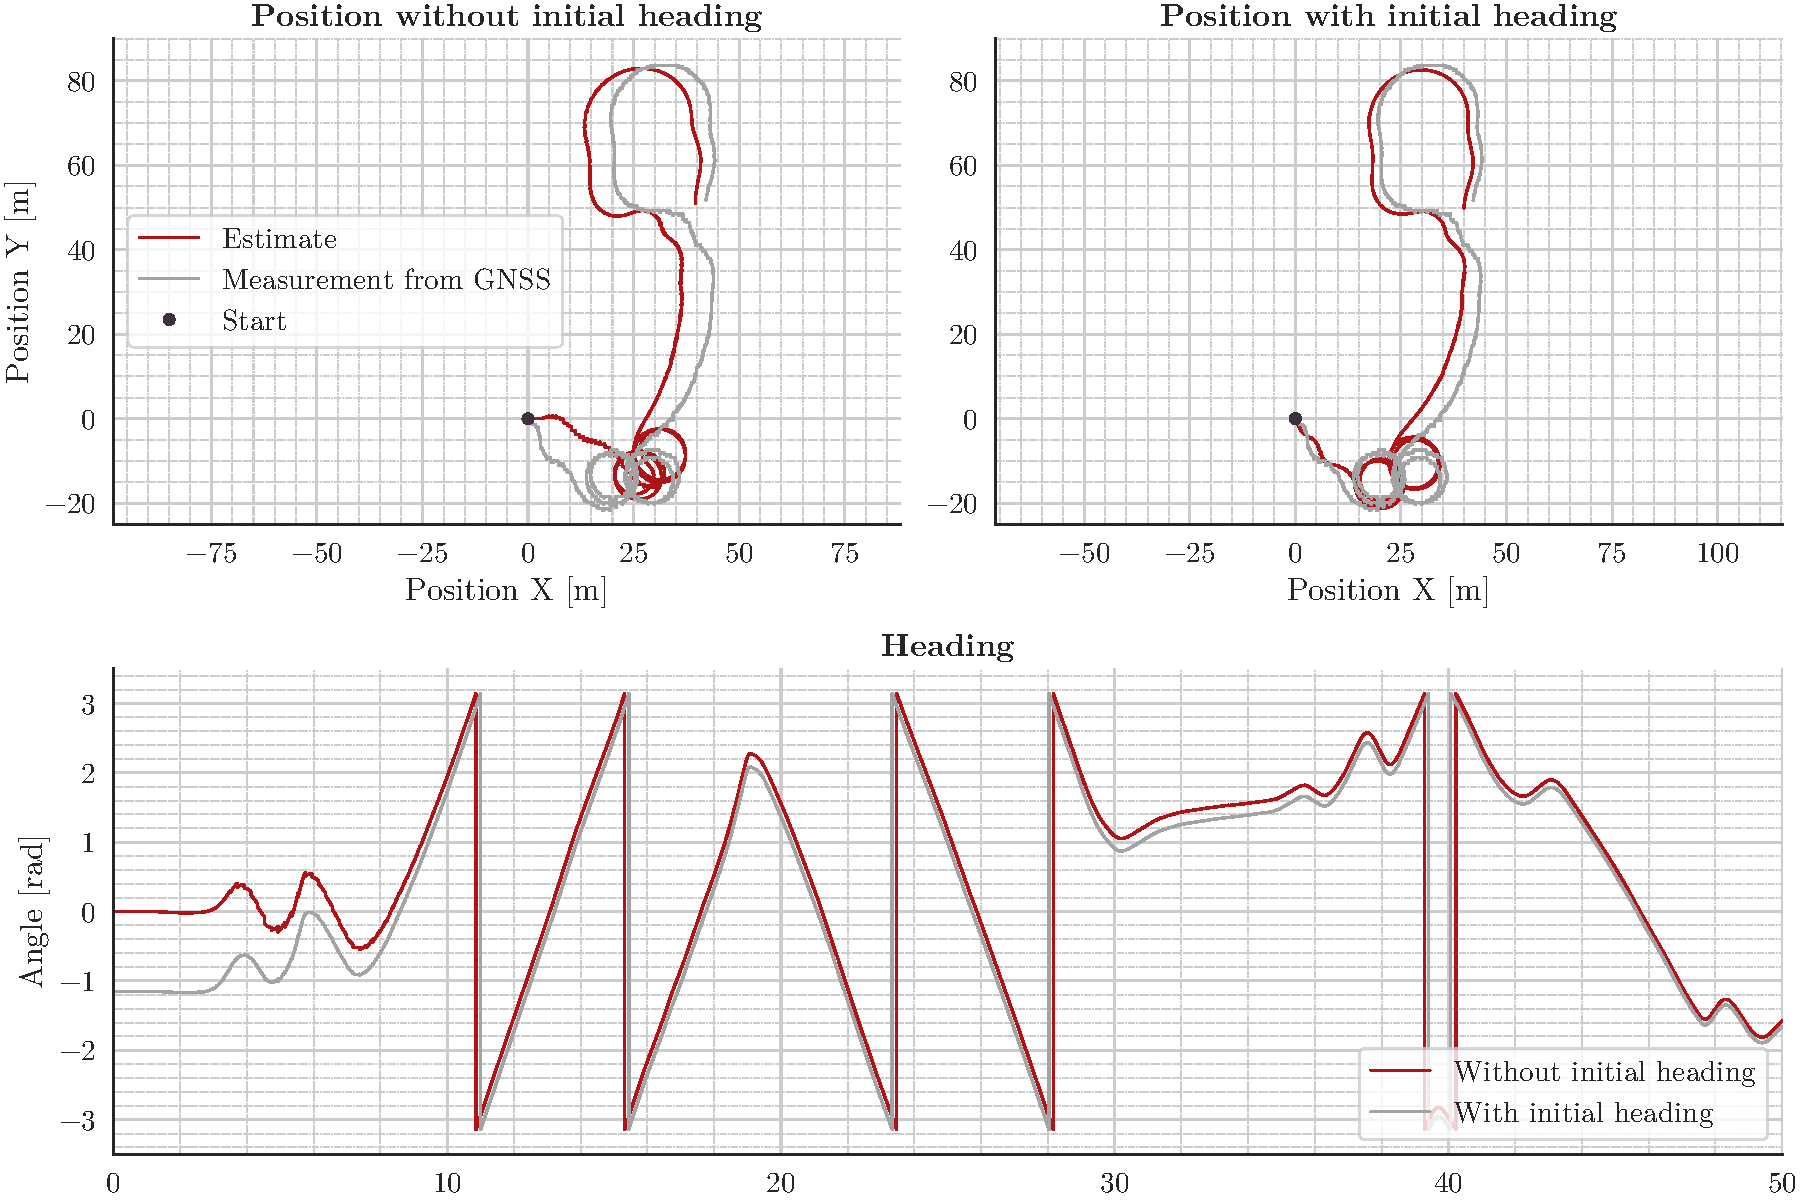
\includegraphics[width=\textwidth]{plot_ekf_pos}%
	\caption{EKF estimate of position and heading}
	\label{fig:ekf-position}
\end{figure}

Since the \gls{ekf} estimate is essentially a weighted average, the result varies with the measurement covariance settings. A detailed sensitivity analysis is beyond the scope of this thesis, but in practice, empirically determined settings should be enough.

\section{Discussion}
The results presented in the previous section show, that the state estimation generally works well and improves the quality beyond what raw measurements could provide. The estimate of the longitudinal velocity when the optical sensor is available is especially robust, an important prerequisite for good \gls{tc} performance. The different sensor setups between \gls{ev} and \gls{dv} remain somewhat of a challenge. The evaluation shows that the position estimation only works well with heading measurements, therefore it might be better use raw \gls{gnss} measurements for the \gls{ev}, since a good position estimate is only relevant for the \gls{dv}. Also, the optical velocity sensor is crucial for a good lateral velocity estimate, but a non-linear single track model instead of the kinematic model might mitigate this problem in case the sensor is unavailable.

However, the state estimation needs more extensive testing in real driving situations, on the one hand to calibrate and parametrize the outlier detection and the \gls{ekf}, on the other hand to see if it generalizes well, since the measurement data used for the simulation are not very diverse. Furthermore, they do not include heading measurements and only two \glspl{imu}. With a third \gls{imu}, the maximum-likelihood-based fusion should be revisited, but with two \glspl{imu}, the mean-based fusion is preferable due to its simplicity and less computational complexity. Lastly, other failure detection approaches such as the median test, chi-squared test and variance test can be evaluated in case the present approaches are insufficient.
